\chapter{Технологический раздел}

\section{Выбор средств разработки}

Для разработки загружаемого модуля ядра выбран язык программирования C. Выбор языка программирования С основан на том, что исходный код ядра Linux, все его модули и драйверы написаны на данном языке.

\section{Добавление перехватчика системных вызовов}

На листинге~\ref{lst:add_interceptor} представлен код добавления обработчика системных вызовов.

\begin{lstlisting}[language=C, label=lst:add_interceptor, caption={Добавление обработчиков системных вызовов}]
static const char symbol_open[MAX_SYMBOL_LEN] = "do_sys_openat2";
static const char symbol_read[MAX_SYMBOL_LEN] = "ksys_read";
static const char symbol_write[MAX_SYMBOL_LEN] = "ksys_write";

static struct kretprobe kretprobes[SYSCALL_NUM] = {
    {
        .handler		= return_handler,
        .entry_handler	= open_entry_handler,
        .data_size		= sizeof(struct syscall_data_t),
        .maxactive		= 64,
    },
    {
        .handler		= return_handler,
        .entry_handler	= read_entry_handler,
        .data_size		= sizeof(struct syscall_data_t),
        .maxactive		= 64,
    },
    {
        .handler		= return_handler,
        .entry_handler	= write_entry_handler,
        .data_size		= sizeof(struct syscall_data_t),
        .maxactive		= 64,
    }
};

static int __init informer_init(void)
{
    int rc;
    int i;
    kretprobes[SYSCALL_OPEN].kp.symbol_name = symbol_open;
    kretprobes[SYSCALL_READ].kp.symbol_name = symbol_read;
    kretprobes[SYSCALL_WRITE].kp.symbol_name = symbol_write;
    for (i = 0; i < SYSCALL_NUM; i++)
    {
        rc = register_kretprobe(&(kretprobes[i]));
        if (rc < 0) {
            printk(KERN_ERR "informer: register_kretprobe failed, returned %d", rc);
            i--;
            while (i >= 0)
            {
                unregister_kretprobe(&(kretprobes[i]));
                i--;
            }
            return -1;
        }
        printk(KERN_INFO "informer: registered return probe at %s: %p", kretprobes[i].kp.symbol_name, kretprobes[i].kp.addr);
    }
    ...
}
\end{lstlisting}

\section{Замер времени исполнения системного вызова}

На листинге~\ref{lst:open} представлен код замера времени выполнения системного вызова open.

\begin{lstlisting}[language=C, label=lst:open, caption={Замер времени выполнения системного вызова open}]
static int open_entry_handler(struct kretprobe_instance *ri, struct pt_regs *regs)
{
    struct syscall_data_t *data;
    if (!current->mm)
        return 1; // Skip kernel threads
    data = (struct syscall_data_t *) ri->data;
    data->entry_timestamp = ktime_get();
    data->syscall_num = SYSCALL_OPEN;
    data->pid = current->pid;
    return 0;
}

static int return_handler(struct kretprobe_instance *ri, struct pt_regs *regs)
{
    s64 duration;
    ktime_t now;
    struct syscall_info_t info;
    struct syscall_data_t *data = (struct syscall_data_t *) ri->data;
    now = ktime_get();
    duration = ktime_to_ns(ktime_sub(now, data->entry_timestamp));
    if (!processes[data->pid].exist)
        processes[data->pid].exist = 1;
    info = processes[data->pid].syscalls[data->syscall_num];
    info.count++;
    info.sum_duration += duration;
    if (info.max_duration < duration)
        info.max_duration = duration;
    processes[data->pid].syscalls[data->syscall_num] = info;
    return 0;
}
\end{lstlisting}

\section{Получение от пользователя PID процесса}

На листинге~\ref{lst:custom_write} представлен код получения PID процесса для вывода информации.

\begin{lstlisting}[language=C, label=lst:custom_write, caption={Получение PID процесса для вывода информации}]
ssize_t custom_write(struct file *file, const char __user *buf, size_t len, loff_t *offp)
{
    printk(KERN_INFO "informer: called write");
    if(kstrtoint_from_user(buf, len, 10, &output_pid))
    {
        printk(KERN_ERR "informer: read int from user error");
        return -1;
    }
    printk(KERN_INFO "informer: saved pid %d to output", output_pid);
    return len;
}
\end{lstlisting}

\section{Вывод информации о процессе пользователю}

На листинге~\ref{lst:read} представлен код вывода статистики системных вызовов для процесса.

\begin{lstlisting}[language=C, label=lst:read, caption={Вывод статистики системных вызовов для процесса}]
void show_syscall(struct seq_file *m, struct syscall_info_t info)
{
    seq_printf(m, "\tmax_duration = %lld ns\n", info.max_duration);
    seq_printf(m, "\tavg_duration = %lld ns\n", info.sum_duration / info.count);
    seq_printf(m, "\tcount = %d\n", info.count);
}
static int seqfile_show(struct seq_file *m, void *v)
{
    printk(KERN_INFO "informer: called show");
    if (!processes[output_pid].exist) {
        seq_printf(m, "No information about PID=%d.\n", output_pid);
        seq_printf(m, "You can change PID via writing it to /proc/syscalls file.\n");
        return 0;
    }
    seq_printf(m, "System calls statistics of PID=%d.\n", output_pid);
    seq_printf(m, "\nopen()\n");
    show_syscall(m, processes[output_pid].syscalls[SYSCALL_OPEN]);
    seq_printf(m, "\nread()\n");
    show_syscall(m, processes[output_pid].syscalls[SYSCALL_READ]);
    seq_printf(m, "\nwrite()\n");
    show_syscall(m, processes[output_pid].syscalls[SYSCALL_WRITE]);
    return 0;
}
\end{lstlisting}

\section{Демонстрация работы модуля}

На рисунке~\ref{img:demo} представлена демонстрация работы модуля ядра.

\begin{figure}[h!]
    \centering
    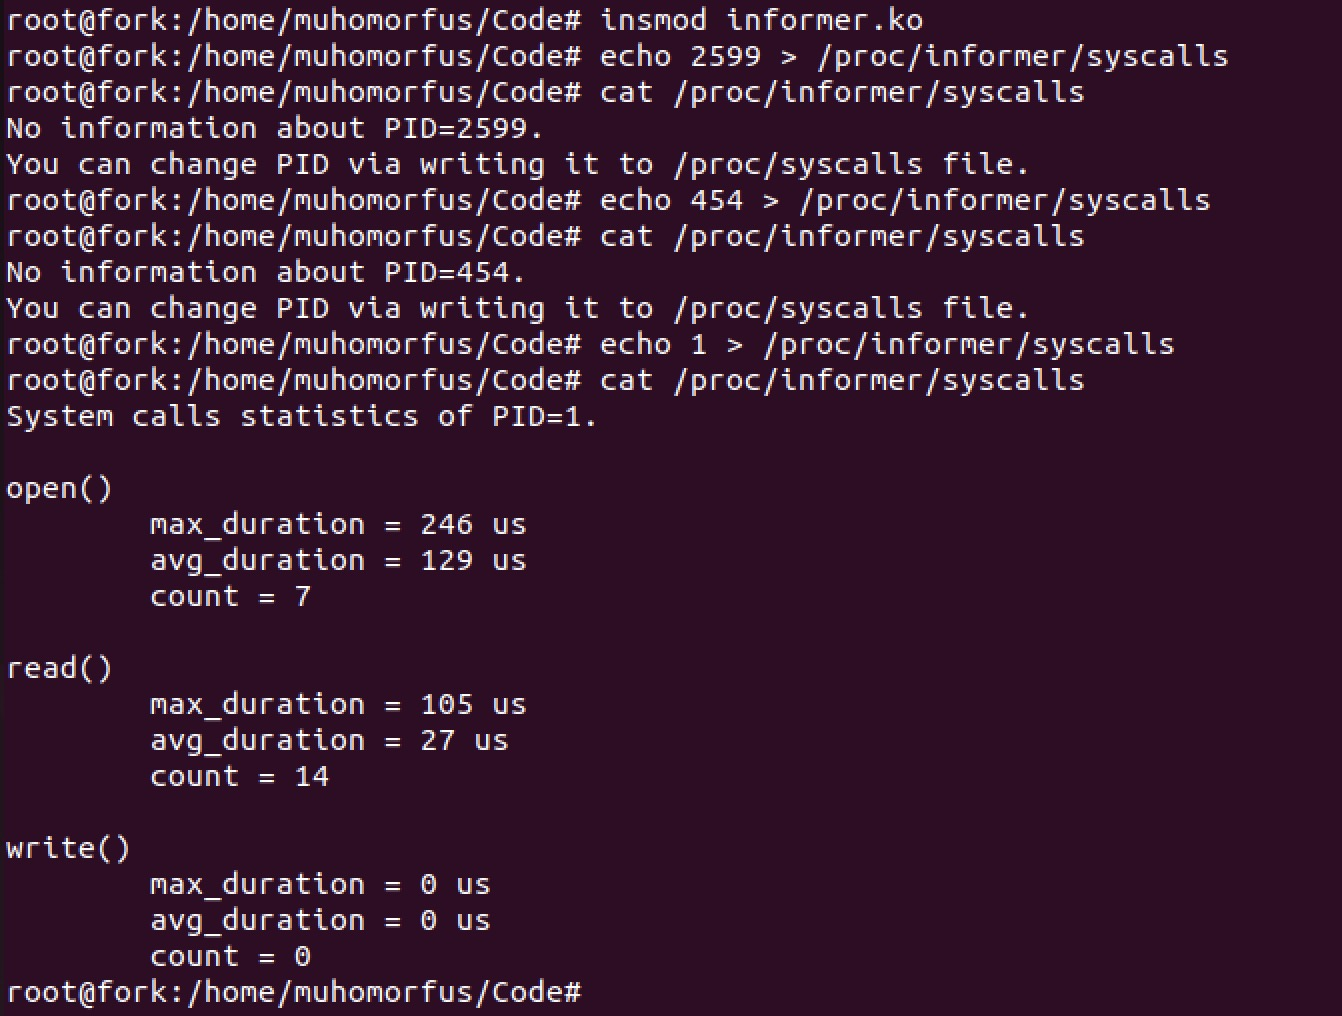
\includegraphics[width=\textwidth]{assets/demo.jpeg}
    \caption{Получение информации о системных вызовах, совершенных процессов}
    \label{img:demo}
\end{figure}

